\documentclass[letterpaper,superscriptaddress,aps,pra,nolongbibliography,twocolumn,showpacs,floatfix,10pt]{revtex4-2} % {{{
% \documentclass[pra]{revtex4-2}
%\usepackage[notref,notci2te]{showkeys} I
%\usepackage[notref]{showkeys}
%\usepackage{setstack}
\usepackage{url}
\usepackage{amsmath}
\usepackage{amssymb}
\usepackage[utf8]{inputenc}
\usepackage[english]{babel}
\usepackage[T1]{fontenc}

\usepackage{ulem}

\usepackage{tikz}
\usetikzlibrary{arrows}


\usepackage{amsmath}
\usepackage{hyperref}
\usepackage{lipsum}
\usepackage{graphicx,helvet}
\usepackage{color}
%\usepackage{bm}                      % added by TG
\usepackage{mathtools}
%\usepackage[inline]{showlabels}
%\usepackage[inner]{showlabels}
\usepackage{bbm,bm}
\usepackage{soul}
\usepackage{amsfonts}
 \usepackage{amsmath}
\usepackage{lipsum}% http://ctan.org/pkg/lipsum
\definecolor{mygray}{gray}{0.4}
\definecolor{light-blue}{rgb}{0.8,0.85,1}
\graphicspath{{figs_avance/}}
\usepackage{amsthm}
%\usepackage{MnSymbol}%
%\usepackage{wasysym}%
%\usepackage{bbm}% bold math
%\usetikzlibrary{decorations.shapes}
\usepackage[draft,inline,nomargin]{fixme} \fxsetup{theme=color}
\newcommand\dsone{\mathds{1}}
\FXRegisterAuthor{cp}{acp}{\color{blue}CP}
\FXRegisterAuthor{fl}{afl}{\color{orange}FL}
\definecolor{jacolor}{RGB}{200,40,0} \FXRegisterAuthor{ja}{aja}{\color{jacolor}JA}
\FXRegisterAuthor{dd}{ddg}{\color{green}DD}
\FXRegisterAuthor{af}{aaf}{\color{magenta}AF}

\newcommand{\esqueletoja}[1]{\textcolor{jacolor}{#1}}


\newcommand{\cuadritotikz}{
% \pgfmathsetmacro{\unitstep}{5.2}
% \node at (-0.5,0.5) {(a)} ;
    \foreach \x in {0,1,2,3} {
      \foreach \y in {0,1,2,3} {
        \begin{scope}[shift={(\x,-\y)}] 
          \draw[black!10] (0,0) rectangle (1,1); 
%           \node at (0.5,0.5) {$\tau_{\y,\x}$};
         \end{scope}
%         \node[block] at (2,-\y) (block\y) {$f_\y$};
%         \draw[->] (block\y.east) -- +(0.5,0);
    }
    }
 \draw (0,-3) rectangle (4,1);
}

\newcommand\todo[1]{\textcolor{red}{#1}}
% \renewcommand\todo[1]{}
%\def\>{\rangle} \def\<{\langle}
\renewcommand{\>}{\rangle}
\mathchardef\Re="023C
\mathchardef\Im="023D
\usepackage[mathlines]{lineno}  
%\linenumbers
 \setlength\linenumbersep{3pt}%\modulolinenumbers[5]
% \newcommand{\red}{\color{red}}
\newcommand{\<}{\langle}
\newcommand{\mele}[2]{\ensuremath{| #1 \rangle \langle #2 |}}
\newcommand{\prj}[1]{\ensuremath{| #1 \rangle \langle #1 |}}
\newcommand{\jami}{Jamiołkowski}
\newcommand{\mcU}{\mathcal{U}}
\newcommand{\mcO}{\mathcal{O}}
\newcommand{\mcI}{\mathcal{I}}
\newcommand{\mcL}{\mathcal{L}}
\newcommand{\mcB}{\mathcal{B}}
\newcommand{\mcH}{\mathcal{H}}
\newcommand{\mcT}{\mathcal{T}}
\newcommand{\mcE}{\ensuremath{\mathcal{E}}}
\newcommand{\mcG}{\ensuremath{\mathcal{G}}}
\newcommand{\mcM}{\mathcal{M}}
\newcommand{\mcN}{\mathcal{N}}
\newcommand{\nnn}{\mathcal{N}}
\newcommand{\choi}{\ensuremath{\mcD}}
\newcommand{\mmm}{\mathcal{M}}
\newcommand{\sss}{\mathcal{S}}
\newcommand{\mcD}{\mathcal{D}}
\newcommand{\mcA}{\mathcal{A}}
\newcommand{\mcP}{\mathcal{P}}
\newcommand{\valpha}{{\vec \alpha}}
\newcommand{\vgamma}{{\vec \gamma}}
\newcommand{\one}{\openone}
\newcommand{\setA}{\ensuremath{{\sf A}}}
\newcommand{\hilbert}{\ensuremath{{\sf H}}}
\newcommand{\spV}{\ensuremath{V}}
\newcommand{\spW}{\ensuremath{W}}
\newcommand{\id}{\text{id}}
\newcommand{\pce}{\ensuremath{\text{PCE}}}
\newcommand{\vbeta}{\vec \beta}
\newcommand{\vlambda}{\vec \lambda}
% \newcommand{\vtau}{\vec \tau}
\newtheorem{theorem}{Theorem}
\newtheorem{definition}{Definition}
\newtheorem{proposition}{Proposition}
\newtheorem{corollary}{Corollary}
\newtheorem{lemma}{Lemma}
\newcommand{\mcQ}{\mathcal{Q}}
% \newcommand{\mcG}{\mathcal{G}}
\newcommand{\mcF}{\mathcal{F}}
\newcommand{\mcK}{\mathcal{K}}
\newcommand{\mcS}{\mathcal{S}}
\newcommand{\ie}{i.e.}
\newcommand{\aka}{a.k.a}
\newcommand{\fmlong}{fuzzy measurements}
\newcommand{\Fmlong}{Fuzzy measurements}
\newcommand{\ipr}{\mathrm{ipr}}
\newcommand{\rmH}{\mathrm{H}}
\newcommand{\rmq}{\mathrm{q}}
\newcommand{\cut}{\mathrm{cut}}
\newcommand{\rmd}{\mathrm{d}}
\newcommand{\rmi}{\mathrm{i}}
\newcommand{\blue}{\color{blue}}
\newcommand{\mcC}{\mathcal{C}}
\newcommand{\cg}{\mcC}
%%%%CG commands
\newcommand{\Loc}[1]{\ensuremath{\Lambda_#1^\text{L}}}
\newcommand{\NoLoc}[1]{\ensuremath{\Lambda_{#1}^\text{NL}}}
\newcommand{\NoLoct}[1]{\ensuremath{\tilde{\Lambda}_{#1}^\text{NL}} }
\newcommand{\fuzzytwo}[1]{\ensuremath{\Lambda_#1^\text{fuzzy}}}
\newcommand{\cgtwo}[1]{\ensuremath{\Lambda_#1^\text{cg}}}
% \newcommand{\tp}{TP}
\newcommand{\hp}{HP}
\newcommand{\Imi}{\imath}
\newcommand{\rmf}{f}
%\newcommand{\eg}{\textit{e.g.} }
%\newcommand{\Eg}{\textit{E.g.} }
\newcommand{\eref}[1]{Eq.~(\ref{#1})} 
\newcommand{\sref}[1]{sec.~\ref{#1}}
\newcommand{\fref}[1]{fig.~\ref{#1}}
\newcommand{\tref}[1]{table~\ref{#1}}
\newcommand{\Eref}[1]{Eq.~(\ref{#1})} 
\newcommand{\Sref}[1]{Sec.~\ref{#1}}
\newcommand{\Fref}[1]{Fig.~\ref{#1}}  
\newcommand{\Tref}[1]{Table~\ref{#1}}
\newcommand{\Or}{\mathord{\mathrm{O}}}
\newcommand{\tr}{\mathop{\mathrm{Tr}}u\nolimits}
% \newcommand{\comm}[1]{{\color{red} #1 }}
\newcommand{\qv}{QV}
\newcommand{\old}{\infty}
\newcommand{\Mmed}{\mcM^{\<\cdot\>}}
\newcommand{\MBLP}{\mcM^{\text{BLP}}}
\newcommand{\MRHP}{\mcM^{\text{RHP}}}
\newcommand{\gs}{GS}
\newcommand{\cptp}{CPTP}
\newcommand{\ket}[1]{{\vert #1 \rangle}}
\newcommand{\bra}[1]{{\langle #1 \vert}}
\newcommand{\proj}[2]{{\vert #1 \rangle \langle #2 \vert}}
\newcommand{\projj}[1]{{\vert #1 \rangle \langle #1 \vert}}
% \newcommand{\cp}{\color{red}   }
\newcommand{\diag}{\text{diag}}

% --------------------------------------- Commands added by JA ------------------------------------
\usepackage{physics}
\usepackage{breqn}
% \newcommand{\paulicomponents}{r_{\alpha_1,\ldots,\alpha_N}}
\newcommand{\paulicomponents}{r_\valpha}
\newcommand{\taus}{\tau_\valpha}
\newcommand{\pceg}{\mcG_{\vec \alpha}}
\newcommand{\appref}[1]{appendix~\ref{#1}}
% 
\def\bbra#1{\mathinner{\langle \! \langle{#1}|}}
\def\kket#1{\mathinner{|{#1}\rangle \! \rangle}}
\def\ddyada#1{\mathinner{|{#1}\rangle\!\rangle\!\langle\!\langle{#1}|}}
\def\ddyad#1#2{\mathinner{|{#1}\rangle\!\rangle\!\langle\!\langle{#2}|}}
\def\bbrakket#1#2{\mathinner{\langle\!\langle {#1}|{#2}\rangle\!\rangle}}
% \newcommand{\R}[1]{\label{#1}\linelabel{#1}}
% \newcommand{\lr}[1]{\lineref{#1}}
% --------------------------------------------------------------------------------------------------------------

%\newcommand{\mimath}{\rmi}
%\newcommand{\into}{\int_0^t \rmd \tau \{\blue [Verbo de la introducción]}int_0^t \rmd \tau'}
%\newcommand{\intoh}{\int_0^t \rmd \tau \int_0^\tau \rmd \tau'}

%\providecommand{\openone}{\leavevmode\hbox{\small1\kern-3.8pt\normalsize1}}

%\newcommand{\eps}{\varepsilon} \newcommand{\trc}{\tr_{\rm c}}
%\newcommand{\tre}{\tr_{\rm e}} \newcommand{\mcH}{\mathcal{H}}
%\newcommand{\mcO}{\mathcal{O}} \newcommand{\mcU}{\mathcal{U}}

\newcommand{\unam}{Universidad Nacional Aut\'onoma de M\'exico, Ciudad de M\'exico 01000, Mexico}
\newcommand{\icf}{Instituto de Ciencias F\'{\i}sicas, Universidad Nacional Aut\'onoma de M\'exico, Cuernavaca 62210, Mexico}
\newcommand{\ifunam}{Instituto de F\'{\i}sica, \unam}
\newcommand{\fisguadalajara}{Departamento de F\'isica, Universidad de Guadalajara, Guadalajara, Jal\'isco, M\'exico}
\newcommand{\sas}{Institute of Physics, Slovak Academy of Sciences, D\'ubravsk\'a cesta 9, Bratislava 84511, Slovakia}
\newcommand{\red}{\color{red}}
\newcommand{\ecfmUsac}{Instituto de Investigaci\'on en Ciencias F\'isicas y Matem\'aticas, Universidad de San Carlos de Guatemala, Ciudad Universitaria, Guatemala 01012, Guatemala}
\newcommand{\affalejandro}{Departamento de Física, CCEN, Universidade Federal de Pernambuco, Recife 50670-901, PE, Brazil}

\newcommand{\shk}{Sherrington-Kirkpatrick}
\newcommand{\syr}{Šimkovic y Ross}

\usepackage{subfigure}

% }}}
\begin{document}
% Title, authors, etc {{{
\title{Avance en el proyecto de
Monte Carlo de cadena de Markov de muchas configuraciones} 
\author{José Alfredo de León} 
\begin{abstract} % {{{
En este documento se presentan los resultados del avance del proyecto. 
Se implementó el método de Monte Carlo de cadena de Markov (MCMC) 
para resolver el modelo de vidrio de espín de \shk{}. La
implementación tiene errores y se deben de corregir antes de 
implementa el nuevo algoritmo MCMCMC propuesto por \syr{} en 
\cite{simkovic2021manyconfiguration}. Se discuten las hipótesis del
error en la implementación y las pruebas realizadas para comprobar 
o refutar dichas hipotesis.
Adicionalmente, el tiempo computacional ocupado para estos 
resultados es considerable para considerar implementar el prototipo 
correcto de la implementación del método MCMC y MCMCMC en 
un lenguaje como FORTRAN.
\end{abstract} % }}}
%%
%\pacs{03.65.Yz, 03.65.Ta, 05.45.Mt}
 
\maketitle
% }}}

\section{Resumen del proyecto}
Se planteó como objetivo implementar el nuevo método de Monte Carlo propuesto
por \syr{}~\cite{simkovic2021manyconfiguration}, llamado método 
de Monte Carlo de cadena de Markov (MCMCMC), y reproducir los resultados 
de \cite{simkovic2021manyconfiguration} en el que se aplica el 
nuevo método al modelo de \shk{} y Fermi-Hubbard. El método MCMCMC 
es una generalización del método de Monte Carlo de cadena de Markov (MCMC) 
en el que la configuración propuesta en cada paso Monte Carlo se propone
una configuración de estados y no un estado sólo.

\subsection{Modelo de \shk{}}
El modelo de \shk{} fue propuesto en 1975 como un modelo de vidrios de espín.
Es un modelo de Ising en el cual se incluyen interacciones entre todos los 
espines de la red. A diferencia del modelo de Ising, en el modelo de \shk{}
se consideran interacciones de largo alcance.
La energía del sistema de espines está dada por 
\begin{align}\label{eq:SK:H}
E\qty(\{J_{jk}\},\{S_j\})=\frac{1}{\sqrt{L}}\sum_{j\leq k}J_{jk}S_jS_k,
\end{align}
donde $J_{jk}$ son los parámetros de interacción modelados como números reales
gaussianos con media cero y varianza igual a uno, $L$ el tamaño de la cadena y
%, siguiendo el trabajo 
%realizado por \syr{} en \cite{simkovic2021manyconfiguration},
$S_k$ los eigenvalores $\{+1,-1\}$. 

\section{Qué se ha hecho}
Hasta el momento se ha implementado el método de Monte Carlo 
de cadena de Markov para resolver el modelo de \shk{} 
en la temperatura crítica $T=1$ y utilizando una cadena de tamaño $L=10^3$.

El objetivo era reproducir el resultado de la gráfica de la Fig. 1
para el método MCMC, es decir, la línea punteada negra.

En la siguiente sección describimos con detalle el algoritmo implementado.

\begin{figure}[h]
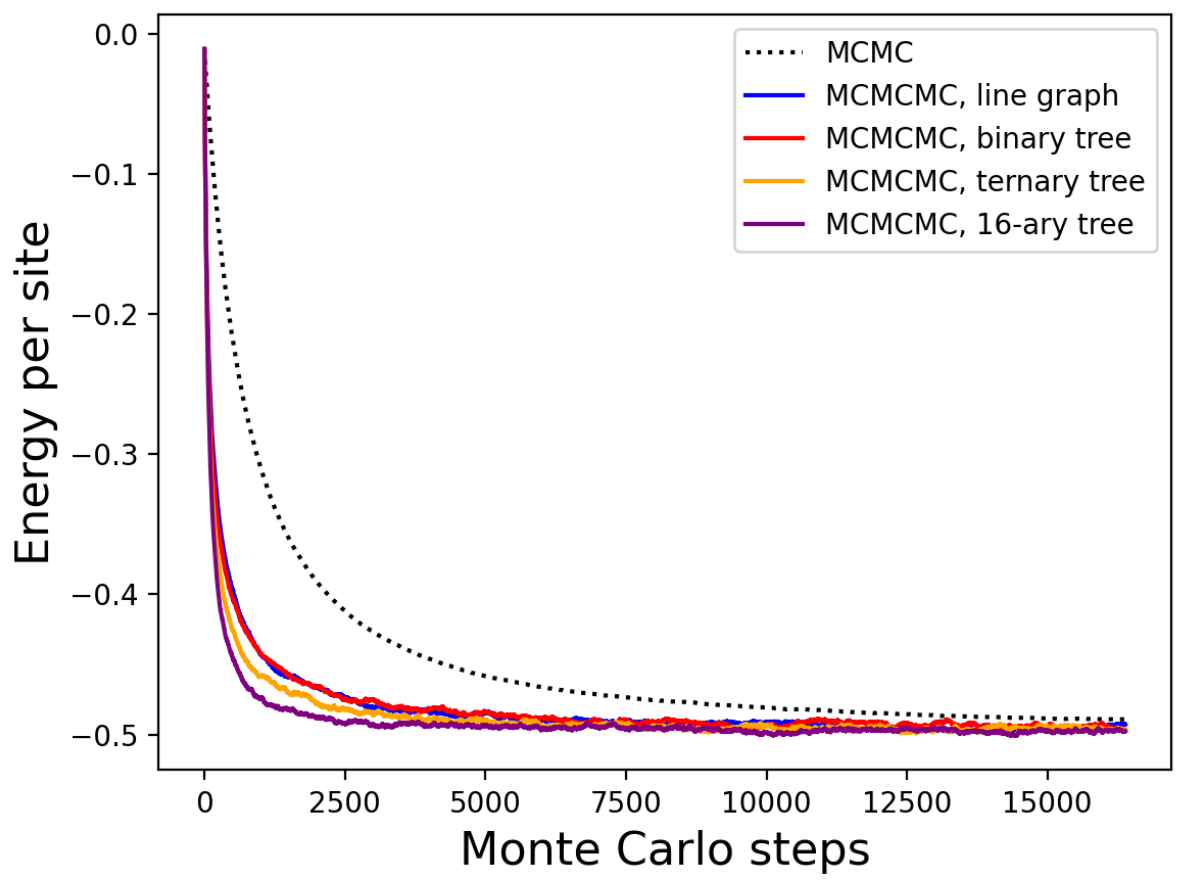
\includegraphics[width=0.95\columnwidth]{resultados}
\caption{Resultados de \syr{} en \cite{simkovic2021manyconfiguration}
para el modelo de \shk{}. Los resultados que se quisieron reproducir 
fue la curva del método MCMC (línea punteada negra).}
\end{figure}

\section{Algoritmo de Metrópolis}
\begin{enumerate}
\item \textbf{Inicializar la configuración}. Se debe inicializar una 
configuración aleatoria antes de comenzar los pasos Monte Carlo.
\begin{enumerate}
\item Generar una configuración aleatoria de $L$ espines $\{ \uparrow,
\downarrow,\downarrow,\uparrow,\ldots,\uparrow\}$.
\item Generar los parámetros de interacción reales $J_{jk}$ con números que 
obedecen una distribución Gaussiana con media 0 y desviación igual a 1.
\item Calcular la energía inicial de la configuración $E_0$, siguiendo
la expresión en \eqref{eq:SK:H}.
\item Elegir aleatoriamente un sitio $s$ para ``voltear'' al espín en 
ese sitio ($\uparrow\ \to\ \downarrow$ o $\downarrow\ \to\ \uparrow$).
\end{enumerate}
\item \textbf{Pasos de Monte Carlo}. Ahora se deberá repetir el paso Monte
Caro hasta que la fluctuación de la energía por sitio ($E/L$) 
sea del orden de $10^{-3}$.
\begin{enumerate}
\item Calcular la energía $E_f$ de la nueva configuración con el espín en el
sitio $s$ invertido.
\item Si $E_f<E_0$, la nueva configuración es aceptada. Si $E_f>E_0$,
entonces la nueva configuración se acepta con una probabilidad de $e^{-(E_f-E_0)/k_BT}$.
\item Escoger un nuevo sitio según una probabilidad Gaussiana con media
igual al sitio anterior y desviación estándar igual a $3$.
Para este paso, se deberán considerar condiciones periódicas.
\end{enumerate}
\end{enumerate}

\section{Resultados}
En las Figs. 2-14 se muestran los resultados obtenidos hasta 
ahora de la implementación descrita en la sección IV. Aún sin comparar
nuestros resultados con los de \syr{} debemos notar que hay un error 
sistemático en nuestra implementación que se muestran en las gráficas dado 
que la energía parece aumentar o mantenerse constante.

Se formularon las siguientes hipótesis sobre el error que ocurre:
\begin{itemize}
\item La probabilidad con la que se acepta una energía $E_f$ mayor 
a la energía de la configuración anterior $E_0$ podría estar incorrecta.
\item La función de distribución que obedece la función para escoger
el nuevo sitio de cada paso Monte Carlo se está escogiendo incorrectamente.
\item En la configuración inicial se están escogiendo desproporcionadamente
más espines en una dirección que en otra.
\end{itemize}

\begin{figure}
\centering
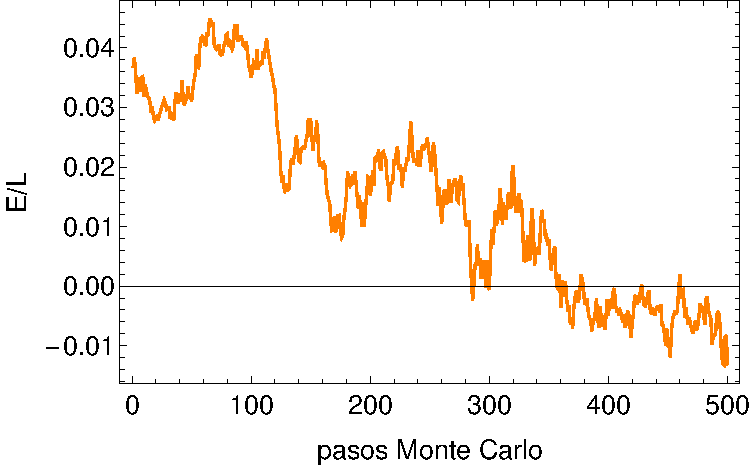
\includegraphics[width=0.9\columnwidth]{intento_001}
\caption{Energía por sitio en función de pasos MC. PDF constante
 para escoger sitio en la nueva configuración.}
\end{figure}

\begin{figure}
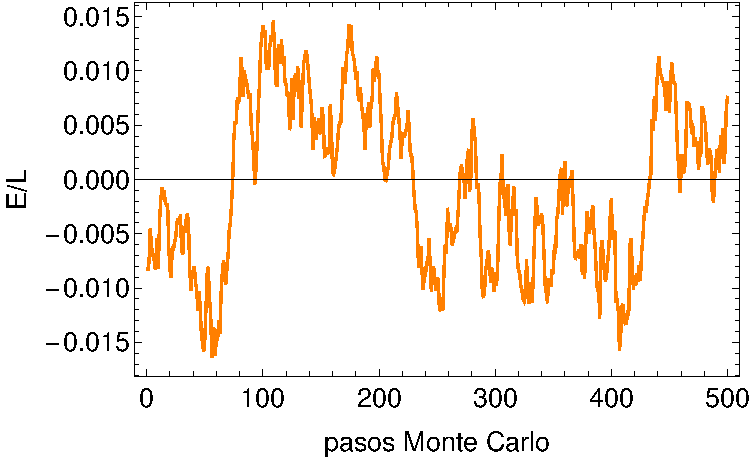
\includegraphics[width=0.9\columnwidth]{intento_002}
\caption{Energía por sitio en función de pasos MC. PDF constante
para escoger sitio en la nueva configuración.}
\end{figure}

\begin{figure}
\centering
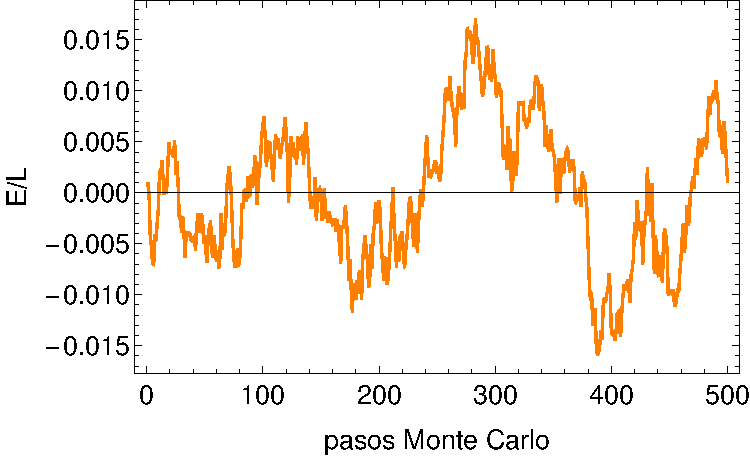
\includegraphics[width=0.9\columnwidth]{intento_003}
\caption{Energía por sitio en función de pasos MC. PDF constante
para escoger sitio en la nueva configuración.}
\end{figure}

\begin{figure}
\centering
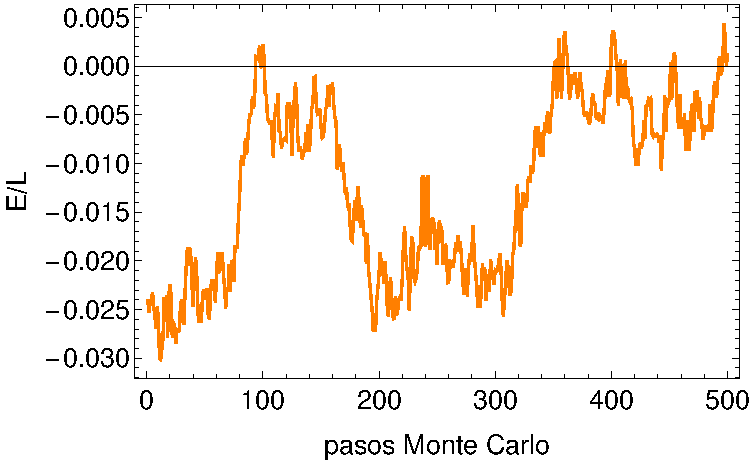
\includegraphics[width=0.9\columnwidth]{intento_004}
\caption{Energía por sitio en función de pasos MC. PDF 
constante para escoger sitio en la nueva configuración.}
\end{figure}
\begin{figure}
\centering
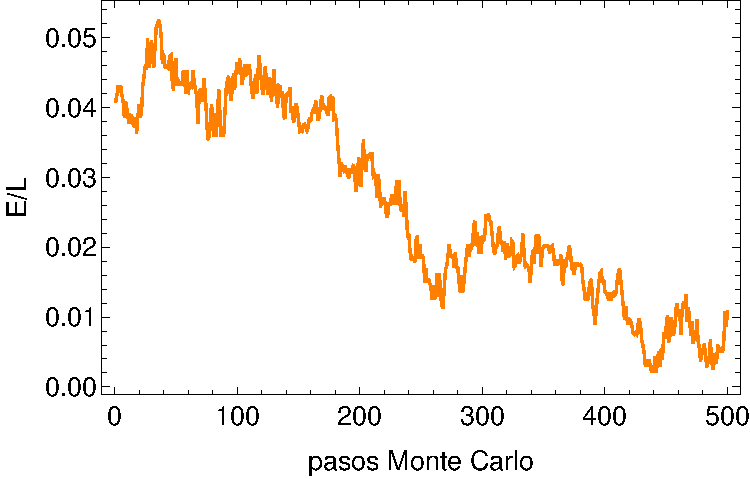
\includegraphics[width=0.9\columnwidth]{intento_005}
\caption{Energía por sitio en función de pasos MC. PDF Gaussiana
con desviación $=$ 2 para escoger sitio en la nueva configuración.}
\end{figure}
\begin{figure}
\centering
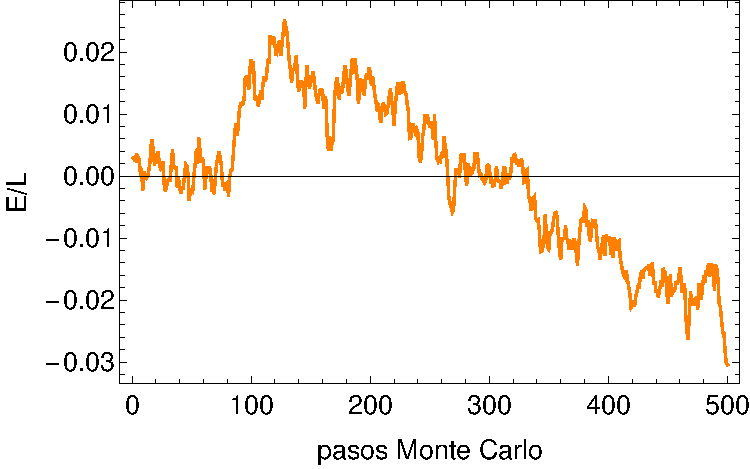
\includegraphics[width=0.9\columnwidth]{intento_006}
\caption{Energía por sitio en función de pasos MC. PDF Gaussiana
con desviación $=$ 5 para escoger sitio en la nueva configuración.}
\end{figure}
\begin{figure}
\centering
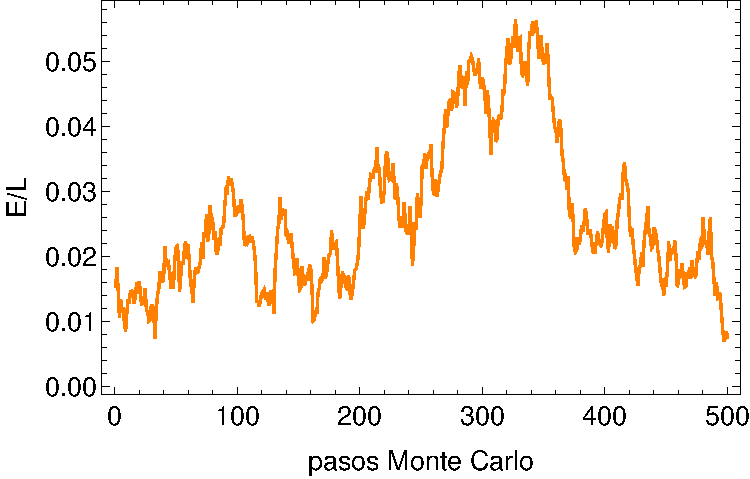
\includegraphics[width=0.9\columnwidth]{intento_007}
\caption{Energía por sitio en función de pasos MC. PDF Gaussiana
con desviación $=$ 10 para escoger sitio en la nueva configuración.}
\end{figure}
\begin{figure}
\centering
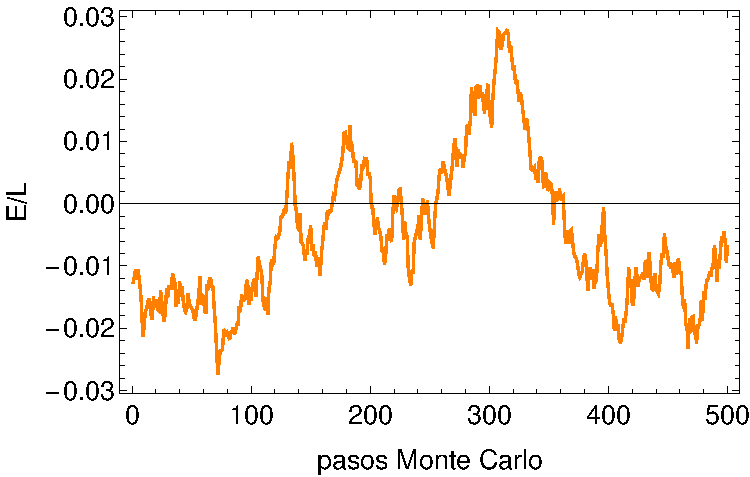
\includegraphics[width=0.9\columnwidth]{intento_008}
\caption{Energía por sitio en función de pasos MC. PDF Gaussiana
con desviación $=$ 50 para escoger sitio en la nueva configuración.}
\end{figure}
\begin{figure}
\centering
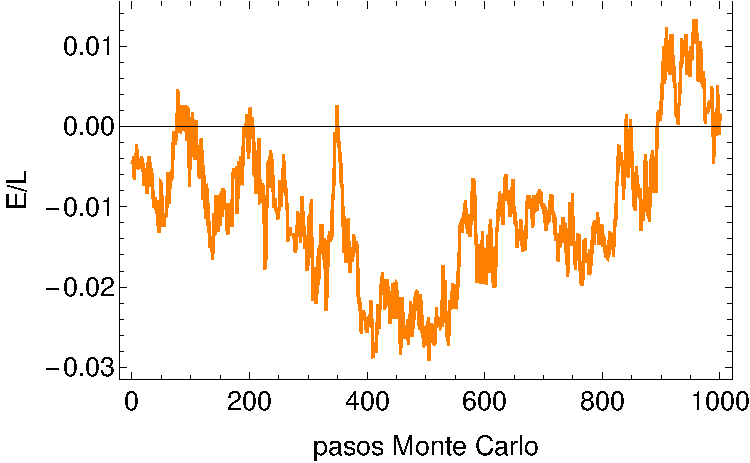
\includegraphics[width=0.9\columnwidth]{intento_009}
\caption{Energía por sitio en función de pasos MC. PDF Gaussiana
con desviación $=$ 3 para escoger sitio en la nueva configuración.}
\end{figure}

\begin{figure}
\centering
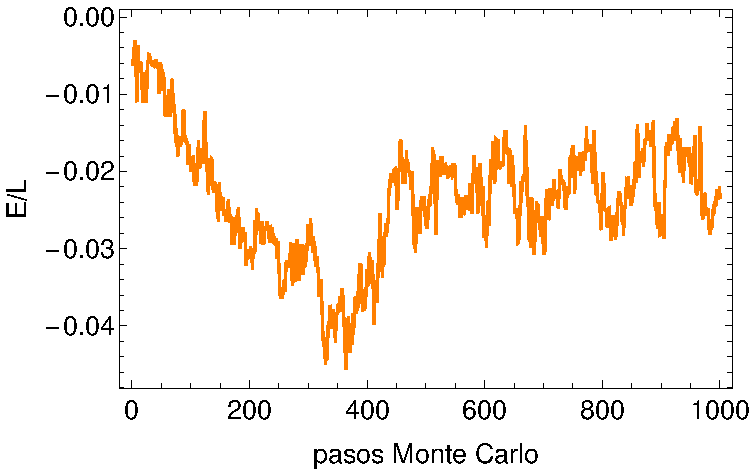
\includegraphics[width=0.9\columnwidth]{intento_011}
\caption{Energía por sitio en función de pasos MC. PDF Gaussiana
con desviación $=$ 2 para escoger sitio en la nueva configuración.}
\end{figure}
\begin{figure}
\centering
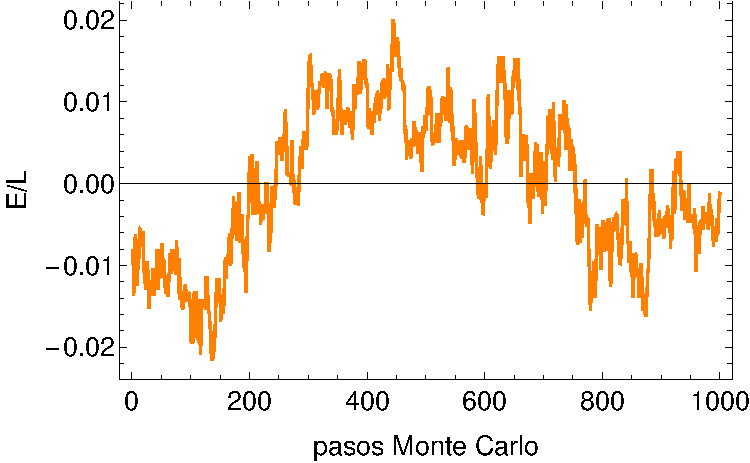
\includegraphics[width=0.9\columnwidth]{intento_012}
\caption{Energía por sitio en función de pasos MC. PDF Gaussiana
con desviación $=$ 2 para escoger sitio en la nueva configuración
y probabilidad es aceptar configuraciones de mayor energía igual a 1/3.}
\end{figure}
\begin{figure}
\centering
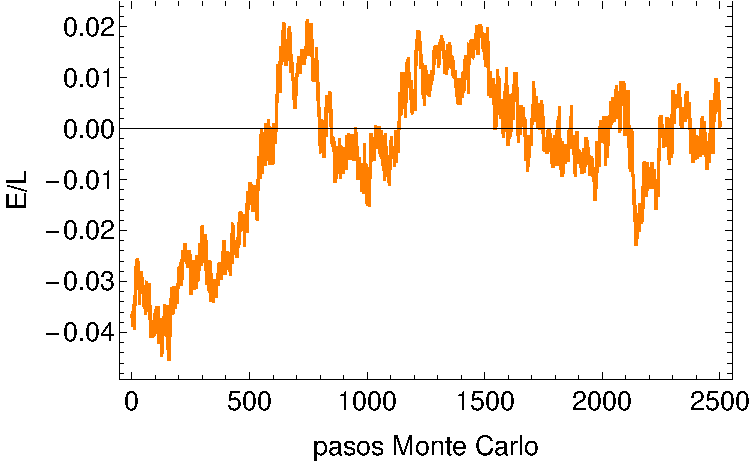
\includegraphics[width=0.9\columnwidth]{intento_013}
\caption{Energía por sitio en función de pasos MC. PDF Gaussiana
con desviación $=$ 3 para escoger sitio en la nueva configuración
y probabilidad es aceptar configuraciones de mayor energía igual a 1/4.}
\end{figure}
\begin{figure}
\centering
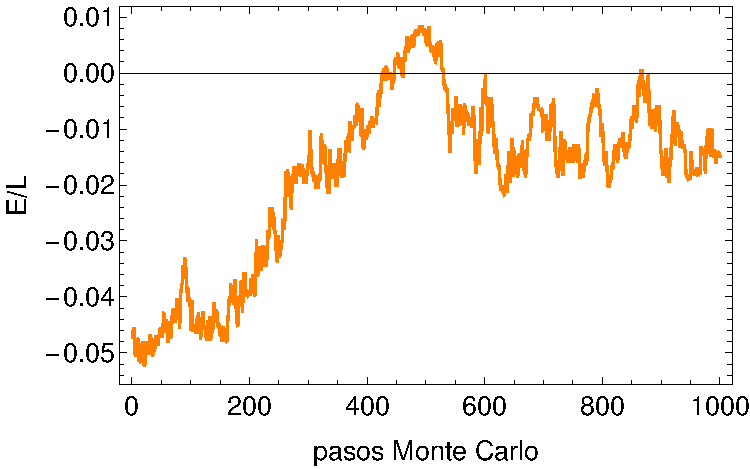
\includegraphics[width=0.9\columnwidth]{intento_014}
\caption{Energía por sitio en función de pasos MC. PDF Gaussiana
con desviación $=$ 5 para escoger sitio en la nueva configuración
y probabilidad es aceptar configuraciones de mayor energía igual a 1/5.}
\end{figure}

%\begin{figure}[h]
%\centering
%\subfigure[$\sigma =$ 2.]{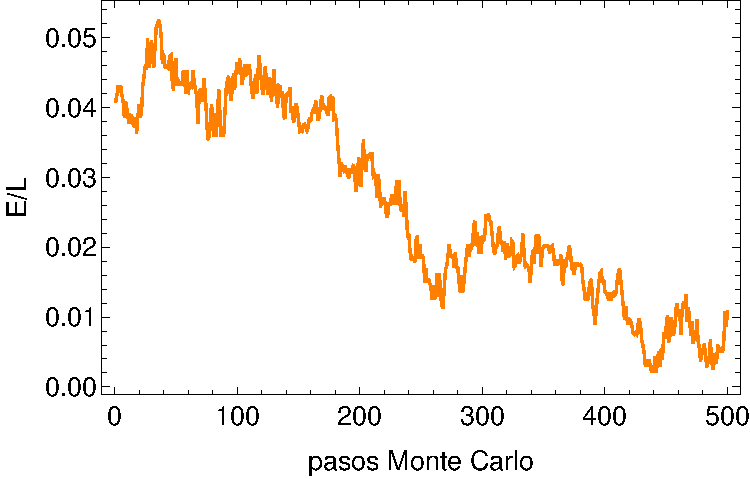
\includegraphics[width=0.9\columnwidth]{intento_005}}
%\subfigure[$\sigma =$ 5.]{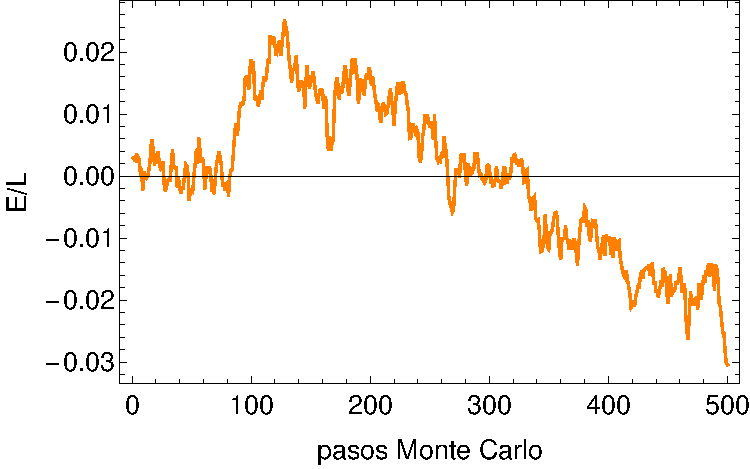
\includegraphics[width=0.9\columnwidth]{intento_006}}
%\subfigure[$\sigma =$ 10.]{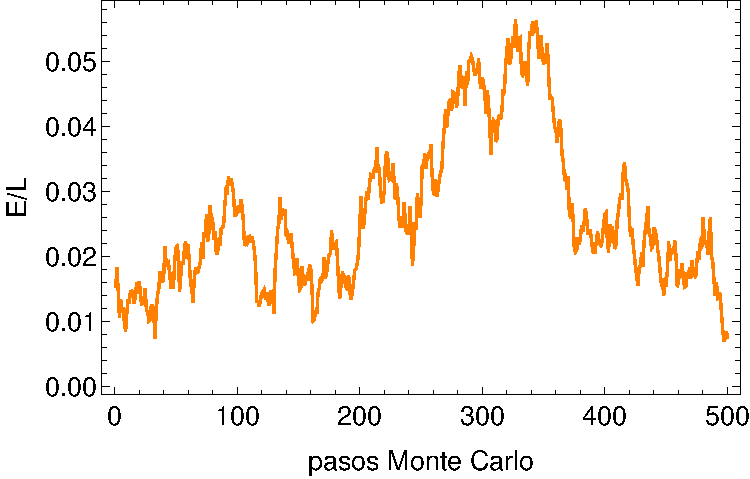
\includegraphics[width=0.9\columnwidth]{intento_007}}
%\subfigure[$\sigma =$ 50.]{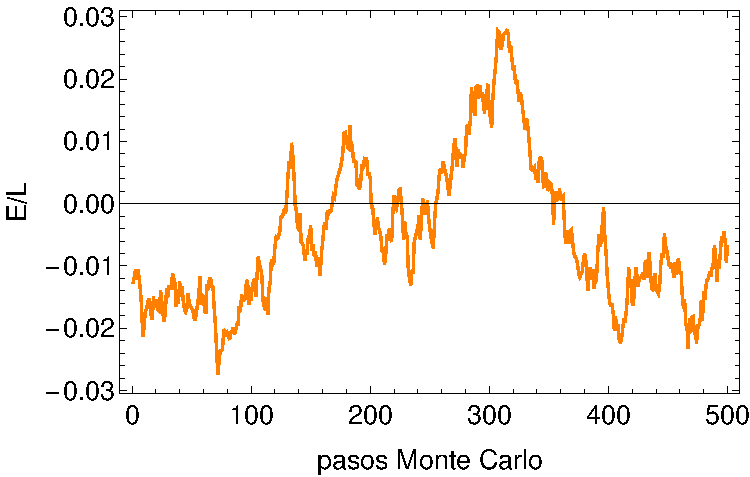
\includegraphics[width=0.9\columnwidth]{intento_008}}
%\caption{Diferentes corridas del método MCMC para el método de \shk{} para 
%diferentes funciones de distribución Gaussiana que siguen los sitios
%nuevos escogidos para diferentes desviaciones estándar.}
%\label{fig:1}
%\end{figure}
%
%\begin{figure}[h]
%\centering
%\subfigure[$\sigma =$ 2.]{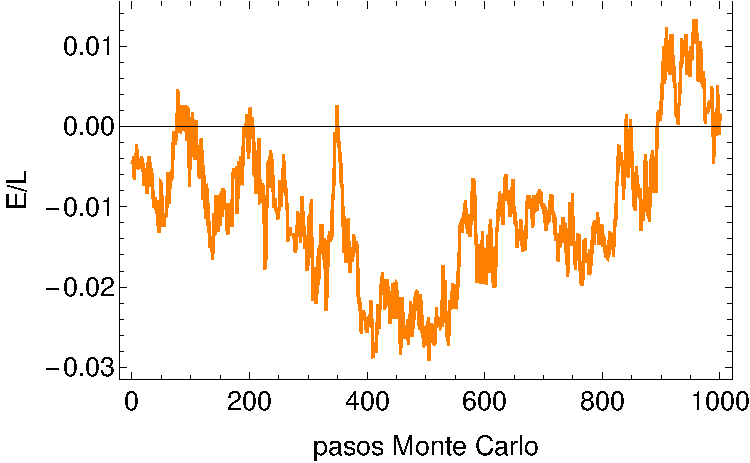
\includegraphics[width=0.9\columnwidth]{intento_009}}
%\subfigure[$\sigma =$ 5.]{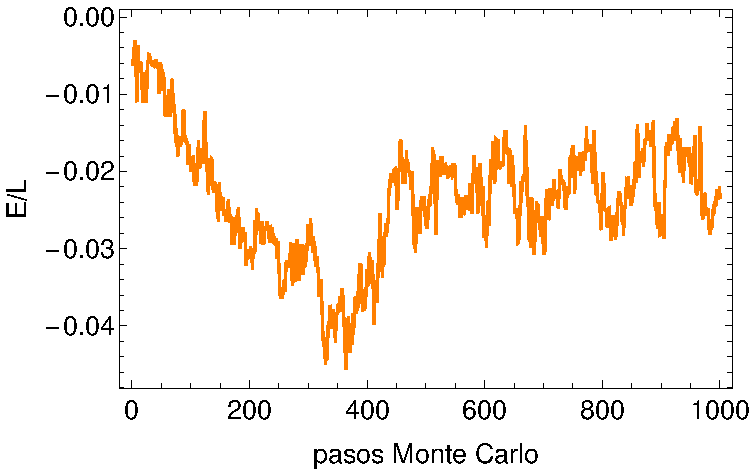
\includegraphics[width=0.9\columnwidth]{intento_011}}
%\subfigure[$\sigma =$ 10.]{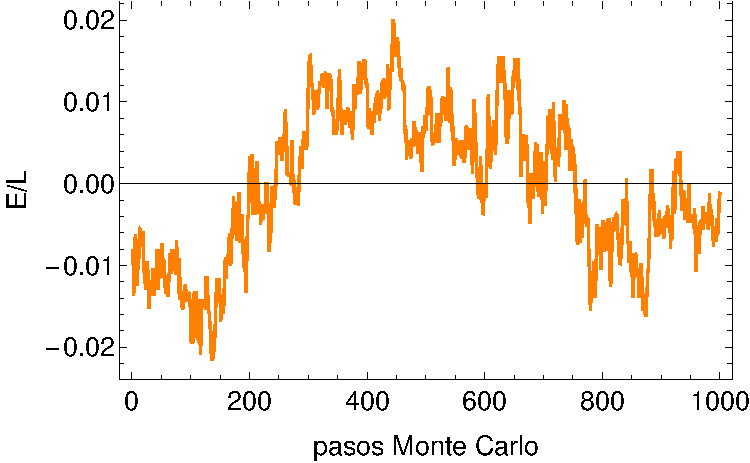
\includegraphics[width=0.9\columnwidth]{intento_012}}
%\subfigure[$\sigma =$ 50.]{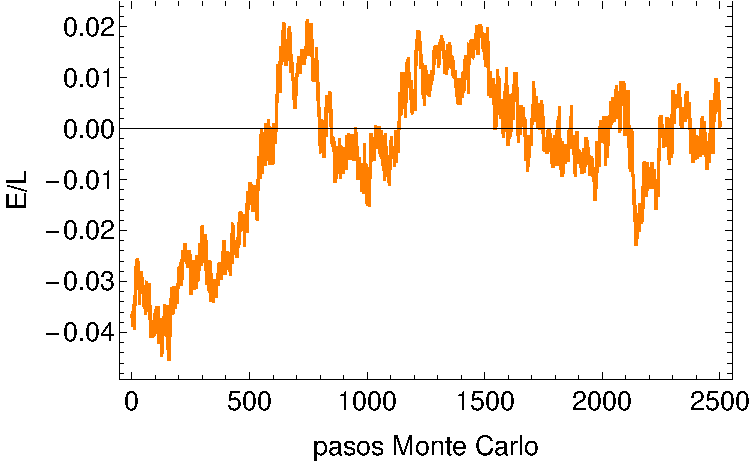
\includegraphics[width=0.9\columnwidth]{intento_013}}
%\caption{Diferentes corridas del método MCMC para el método de \shk{} para 
%diferentes funciones de distribución Gaussiana que siguen los sitios
%nuevos escogidos para diferentes desviaciones estándar.}
%\label{fig:1}
%\end{figure}

Ahora vamos a comentar sobre cada una de las hipóteis formuladas. Nuestras
gráficas de las Figs 2-14 muestran sistemáticamente que nuestra implementación
hace que la energía se mantenga constante o aumente en la mayoría de los casos,
lo cual nos llevó a pensar que la probabilidad con la que se acepta 
un paso MC que aumenta la energía es siempre muy grande, por lo tanto,
se acepta la mayoría de los casos y está siendo contraproducente para 
la convergencia de la energía. Por esta razón, se corrieron pruebas
modificando la probabilidad con la que se acepta un paso MC cuando la 
nueva configuración aumenta la energía a valores constantes de $1/3$, $1/4$
y $1/5$. Sin embargo, las gráficas en la Figs. 12-14 muestran que 
el problema no se solucionó de esa manera, lo que nos llevó a inspeccionar
las otras hipótesis.

Inicialmente, en el paso MC de la implementación de las gráficas en la Figs. 
2-5
se escogía el sitio para invertir el espín con una función de distribución
de probabilidad constante, es decir, todos los sitios en la red eran igual
de probables de escogerse. Posteriormente, se modificó la función de 
distribución para escoger únicamente a los vecinos próximos del sitio
anterior. No obstante, la energía seguía sistemáticamente haciéndose
constante o aumentando. Lo último que se intentó fue considerar una
función de distribución Gaussiana alrededor del sitio escogido anteriormente.
Los resultados no son concluyentes para asegurar o refutar que el 
inconveniente sea la función de distribución de probabilidad con la que 
se escoge cada nuevo sitio en cada paso MC.

Por último, se verificó que la función de distribución de la cual se 
escogía la configuración inicial fuese constante, de tal manera que 
aproximadamente el 50\% de los espines se escojan en una dirección y 
el otro 50\% en la otra.

En lo que inmediatamente sigue en el proyecto deberá de detectarse cuál
es el error en la implementación del método MCMC antes de implementar
el método MCMCMC. Debe también de comentarse que el tiempo de ejecución, 
aunque no se miidió sistemáticamente ni se presentan los resultados aquí,
es de algunos minutos para hacer más de 2000 pasos Monte Carlo para 
una red de 1,000 sitios. Por esa razón, para alcanzar el tamaño de la red
de $2^{10}$ y más de 10,000 pasos MC podría ser deseable implementar 
el método en un lenguaje no interpretado, como FORTRAN.


En resumen, se debe de revisar una vez más la implementación del método
MCMC, implementarlo en un lenguaje no interpretado para poder hacer un 
prototipo de implementación del método MCMCMC, que es el objetivo de 
este proyecto. 

%\janote{comentar que puede ser una buena idea usar otro lenguaje}
%
%\janote{estatus cronograma?}

\bibliographystyle{unsrt}
\bibliography{references}

\end{document}
